\section{Modélisation conceptuelle}\label{sec:concept}

\subsection{Axes de modélisation}
Notre travail de modélisation se heurte à deux verrous scientifiques, identifiés en section \ref{sec:scien} puis développé dans les chapitre \ref{chap:omod} et \ref{chap:mav}, que nous reformulons en : 
\begin{liste}
 	\item[(\g{$\beta$})] \g{l'articulation de plusieurs ensembles de connaissances} [\e{B1 : autonomie}, \e{B2 : réutilisabilité}]. 
 	On distingue ainsi deux ensembles de connaissances : 
 	% à quoi servent-ils ?
 	\begin{listeni} 
 		\item[($\beta_1$)] l'organisation du \e{processus de production audiovisuelle}, qui décrit la répartition des tâches et  les capacités des \e{contributeurs}.
 		Cet ensemble permet d'associer les connaissances fabriquées par les contributeurs aux documents et de faciliter leur implication et les échanges de connaissances.
 		
 		\item[($\beta_2$)] l'organisation du \e{document audiovisuel}, c'est-à-dire sa structure documentaire, le \e{matériel audiovisuel} qu'on y attache et une description de la fabrication de ce matériel (l'\e{écriture audiovisuelle} présente dans le script).
 		Cet ensemble permet de faciliter la recherche, la gestion et donc la réutilisation des fragments audiovisuels.
 	\end{listeni}

 	\item[(\g{$\alpha$})] et \g{une pro(duction/con)sommation progressive et contributive de ces connaissances} [\e{A1: multi-jargon}, \e{A2 : documentation}, \e{A3 : évolution, gestion}].
 	Il s'agit ici du problème de l'évolution et du partage des connaissances liées à un document/fragment audiovisuel tout au long de son ou de ses cycle(s) de vie. 
 	On distingue deux écueils nouveaux suite à l'ouverture de la chaîne à des pratiques de réutilisation : la \e{progressivité de la description}, et la nécesssité de la rendre compréhensible malgré l'\e{hétérogénéité des contributeurs} : 
 	\begin{listeni}
 		\item[($\alpha_1$)] \e{les connaissances sur les document/fragments audiovisuels évoluent et s'ajustent au contexte de production ou de réutilisation}.
 		Les connaissances fabriquées en début de chaîne de production prescrivent un résultat attendu, or de nombeux éléments sont susceptibles d'être modifiés ou précisés par la suite.
 		Il faut donc ajuster les connaissances prescriptives à la réalité des opérations, afin de décrire les résultats effectifs (et non plus l'attendu).
 		Cet écueil apparent est en réalité une opportunité, car la fabrication des descriptions peut alors s'appuyer sur les connaissances prescriptives et les vérifier. 
		De plus, la réutilisation d'un fragment/document audiovisuel dans un nouveau contexte n'implique pas seulement un transfert de matériel audiovisuels, mais également un transfert des connaissances. % mais est-ce que l'on traite vraiment ce cas ? on gère des ensembles de connaissances qui peuvent évoluer (enrichissement)
		Ce transfert peut nécessiter d'extraire certaines connaissances toujours pertinentes et de les associer à celles du nouveau contexte d'utilisation, ou bien de les intégrer à une conceptualisation propre à ce contexte (spécialisation ou bien extension).
		% Cette évolution est rendue possible par 

		\item[($\alpha_2$)] \e{adapter la forme d'expression des connaissances en fonction de l'implication du contributeur dans la chaîne de production et de ses capacités.}
 		Le problème de l'accès aux connaissances est traité par la composition d'une vue contextuelle et spécifique à chaque contributeur de la chaîne, ou chaque groupe de contributeurs.
 		Toute connaissance exprimée à travers le modèle doit pouvoir être caractérisée suivant les codes d'écritures utilisés, eux-mêmes reliées aux capacités des contributeurs.
		Il est alors possible d'effectuer une double sélection ; les connaissances pertinentes suivant l'implication dans la chaîne (en utilisant la description du processus de production); les formes d'expression facilitant leur compréhension (à partir d'une description des capacités des contributeurs).
		% Cette adaptation est rendue possible par le couplage entre conceptualisation, terminologie et documentation.
 	\end{listeni}
\end{liste}


% (\ref{sec:cdc-av}). 



% Par ailleurs, les objectifs métiers de réutilisation ouvre la chaîne de production à de nouveaux contributeurs, dont les niveaux de compétences et de compréhension sont variables (\ref{sec:cdcf}). 
% Les connaissances liées à la production doivent être rendues accessibles à toutes les contributeurs de la chaîne, de même qu'ils doivent contribuer à la fabrication de ces connaissances, tout autant que la fabrication d'objets audiovisuels ou de documents métiers. 

% L'approche que nous avons suivi se positionne sur deux axes de modélisation : 
% \begin{liste}
% 	\item[\g{$\alpha$}] articuler une modélisation conceptuelle aux problèmes de partage et de construction de connaissances communes d'une chaîne de production audiovisuelle ouverte et hétérogène. 
% 	Nous traitons dans cet axe les problèmes définis dans le chapitre \ref{chap:omod} sur la nécessité de construire des terminologies multi-jargon [\g{A1}], d'enrichir une conceptualisation avec de la documentation [\g{A2}], et de gérer l'évolution des unes et des autres de manière indépendantes [\g{A3}].
% 	
	% Nous constatons que les modèles étudiées ne permettent pas de 


% 	\item[\g{$\beta$}]
% \end{liste}



% \subsubsection{Stratégie de description continue}
\begin{figure}[ht!]
\centering
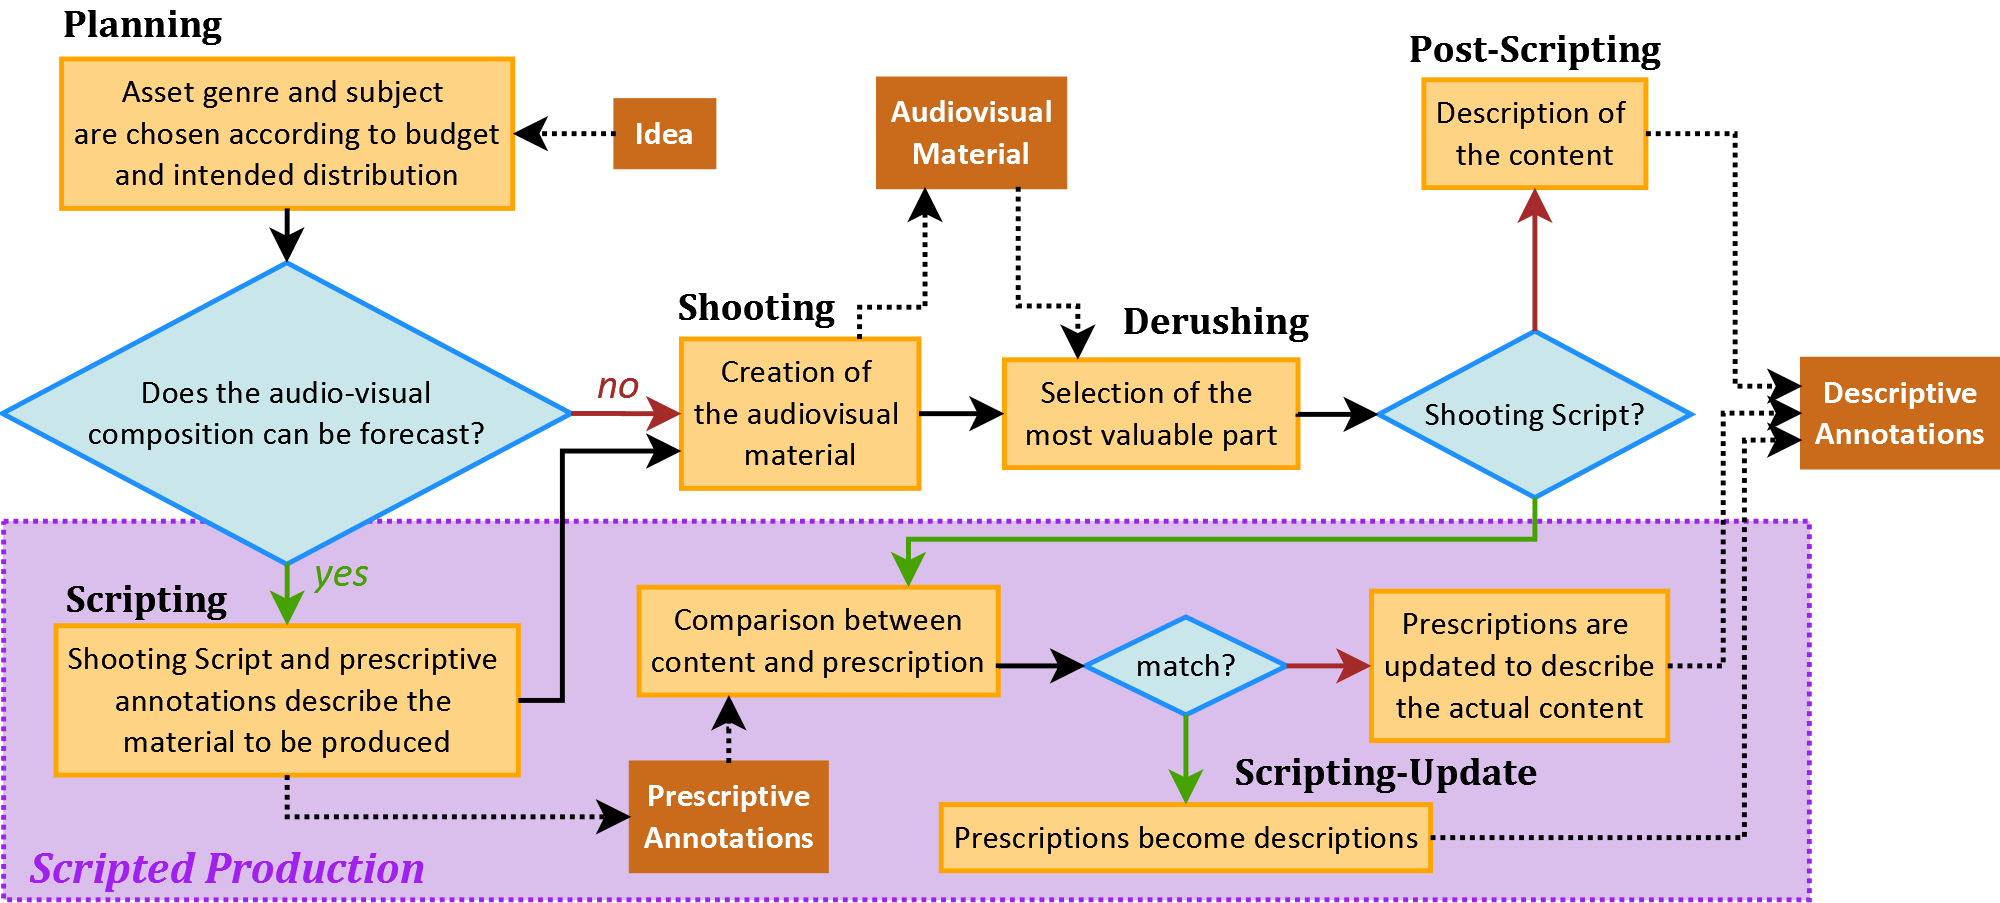
\includegraphics[width=0.9\textwidth]{./images/Approach-Logigram-v2.png}
\caption{}
\label{img:strat-annot}
\end{figure}

\subsubsection{Articuler modélisation conceptuelle et terminologie}%pour favoriser l'accès aux connaissances métiers


\subsubsection{Articuler fabrication d'objets et de connaissances}%pendant la chaîne de production




\subsection{Prise en compte du multi-jargon}\label{}

\subsubsection{Concept et termes}\label{sec:onter}
Le modèle concept-terme que nous avons développé étend la représentation de la terminologie à son contexte d'accès, voir \cite{Diemert2010} et \cite{Diemert2011a}. Dans un premier temps, on associe à chaque concept un ou plusieurs termes, une définition voire une illustration. Chaque terme est caractérisé par son appartenance à une ou plusieurs notations qui représentent une langue, un vocabulaire métier, un code d'écriture, etc. Les fichiers peuvent être caractérisés de manière équivalente, voir figure \ref{img:mj-ct}.


\begin{figure}[ht!]
\centering
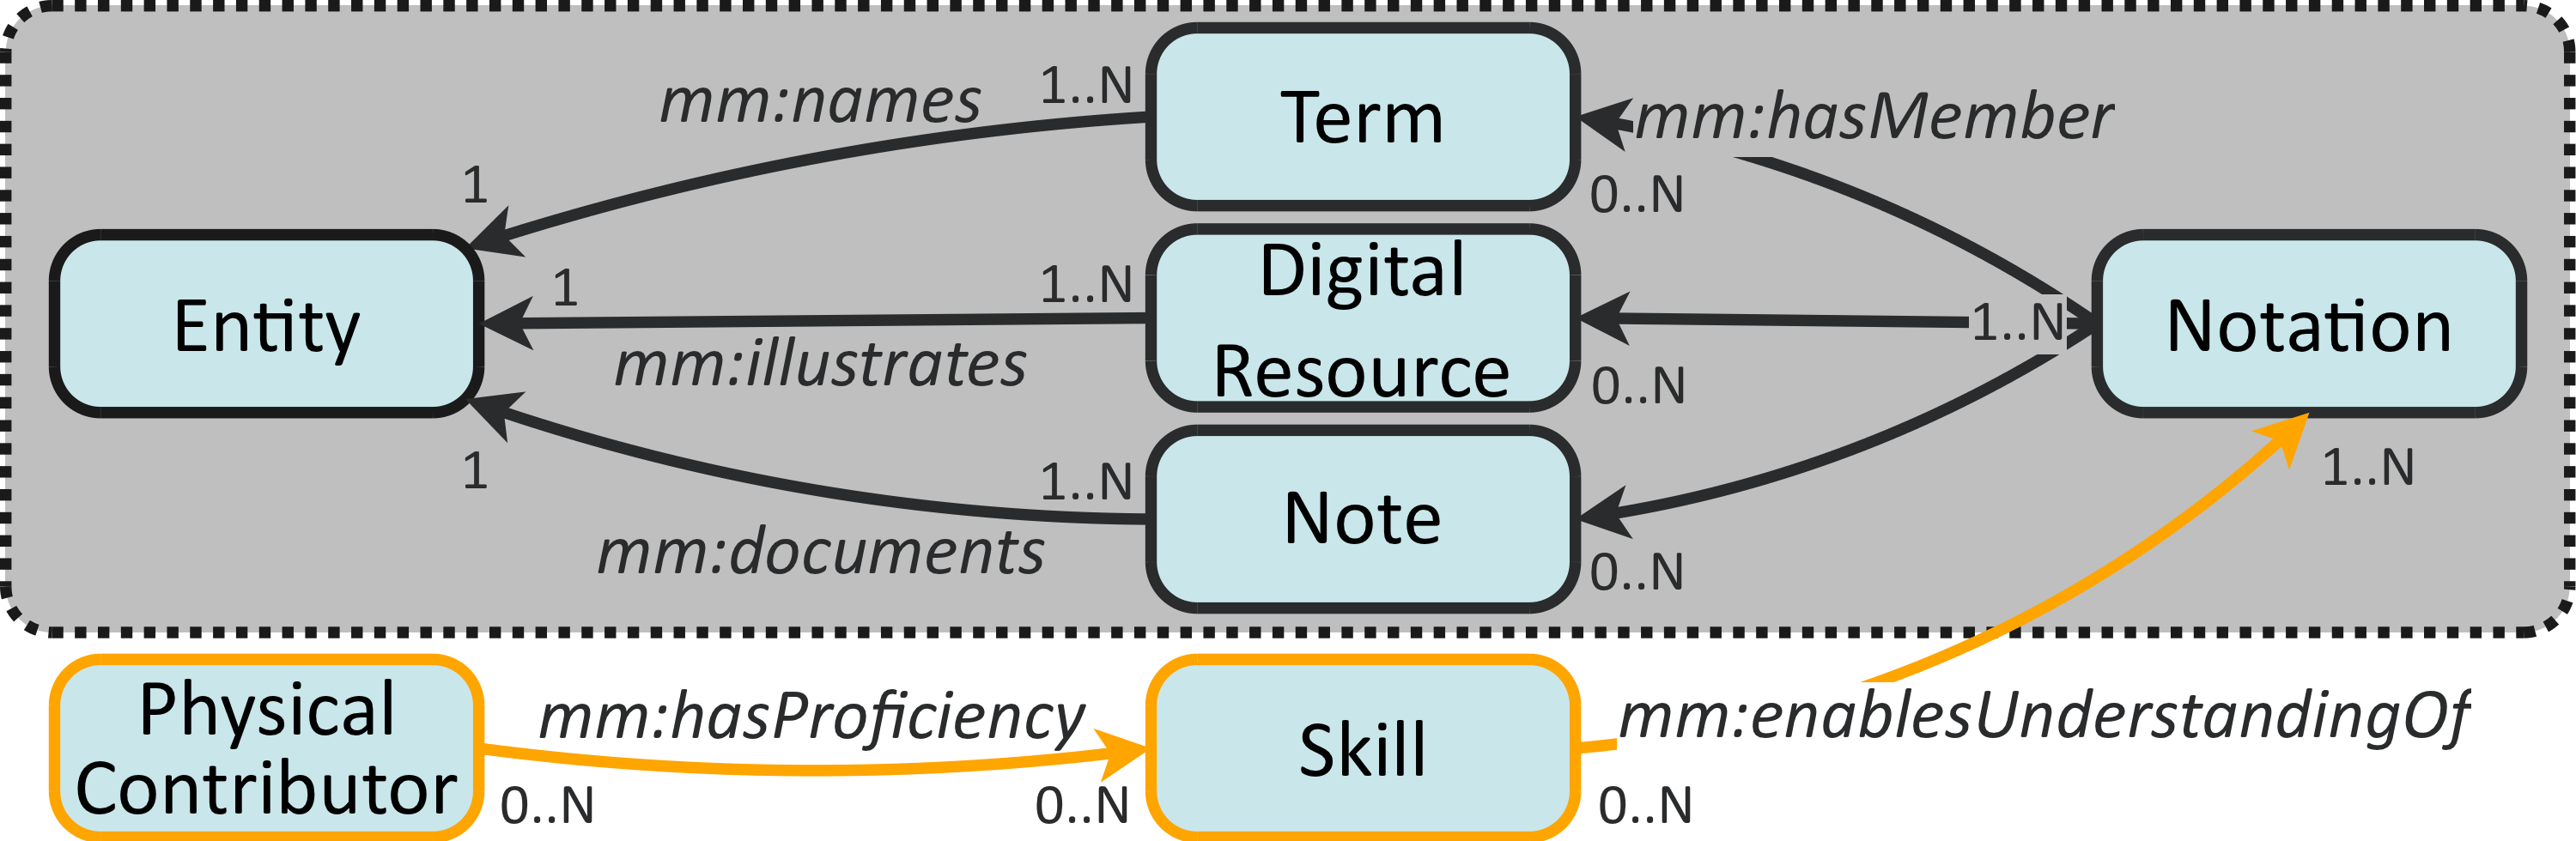
\includegraphics[width=0.75\textwidth]{./images/MOD-TermConcept-v5a.png}
\caption{}
\label{img:mj-ct}
\end{figure}


% \begin{cadrecol}{LightGoldenrodYellow}
	\con{Entity} représente un concept auquel on peut associer
		un terme (\con{Term} -- \rel{mm:names} / \rel{mm:isNamedBy}) ; une ressource média (\con{DigitalResource} -- \rel{mm:illustrates} / \rel{isIllustratedBy}) ou bien une note de documentation (\con{Note} -- \rel{mm:documents} / \rel{is\-Docu\-mentedBy}).
% \end{cadrecol}

% \begin{cadrecol}{LightGoldenrodYellow}
	\con{Term} représente un terme portant une valeur lexicale que l'on peut associer à un concept via la relation \rel{mm:names}.
	Un \con{Term} est caractérisé par son appartenance à un type de \con{Notation} (\rel{mm:isMemberOf} / \rel{mm:hasMember}).
% \end{cadrecol}

% \begin{cadrecol}{LightGoldenrodYellow}
	\con{Notation} représente une caractéristique commune d'un ensemble de \con{Term} ou de ressource numérique \con{DigitalResource}. 
	Il s'agit par exemple d'une langue, d'un format de fichier, d'un type d'encodage de date ou bien d'une structure terminologique propre à une communauté de pratiques ou une communauté d'utilisateurs.
	Chaque \con{Term} peut être décrit par une ou plusieurs \con{Notation}, chacune spécifiant une caractéristique particulière.
	Par exemple, l'étiquette \e{Plan américain} peut être décrite come appartenant à la langue française ainsi qu'à une liste d'autorité de types de plan.
	On distingue quatre types de \con{Notation} : 
	\begin{liste}
		\item \con{NaturalLanguage} représente les langues humaines.
		\item \con{SyntaxEncodingScheme} représente un codage de l'information comme l'encodage des caractères ou bien un format de fichier. 
		\item \con{AuthorityList} représente une liste d'autorité composé de termes. 
		\item \con{VocabularyEncodingScheme} (VES) représente un SOC ou un jargon propre à une organisation ou un métier.\\
	\end{liste}

% \end{cadrecol}


\paragraph{Documentation}
% \begin{cadrecol}{LightGoldenrodYellow}
	\con{Note} représente une chaîne lexicale dont le but est de documenter un concept (\con{Entity}). 
	Nous définissons des spécialisations de \con{Note} à la manière de SKOS, par exemple pour la définition d'un concept (\con{DefinitionNote}). 
% \end{cadrecol}

\con{DigitalResource} représente un fichier numérique. Par exemple, un fichier texte, une photo ou bien un son. 



\subsubsection{Conceptualisation et bases de connaissances}\label{}
\begin{figure}[ht!]
\centering
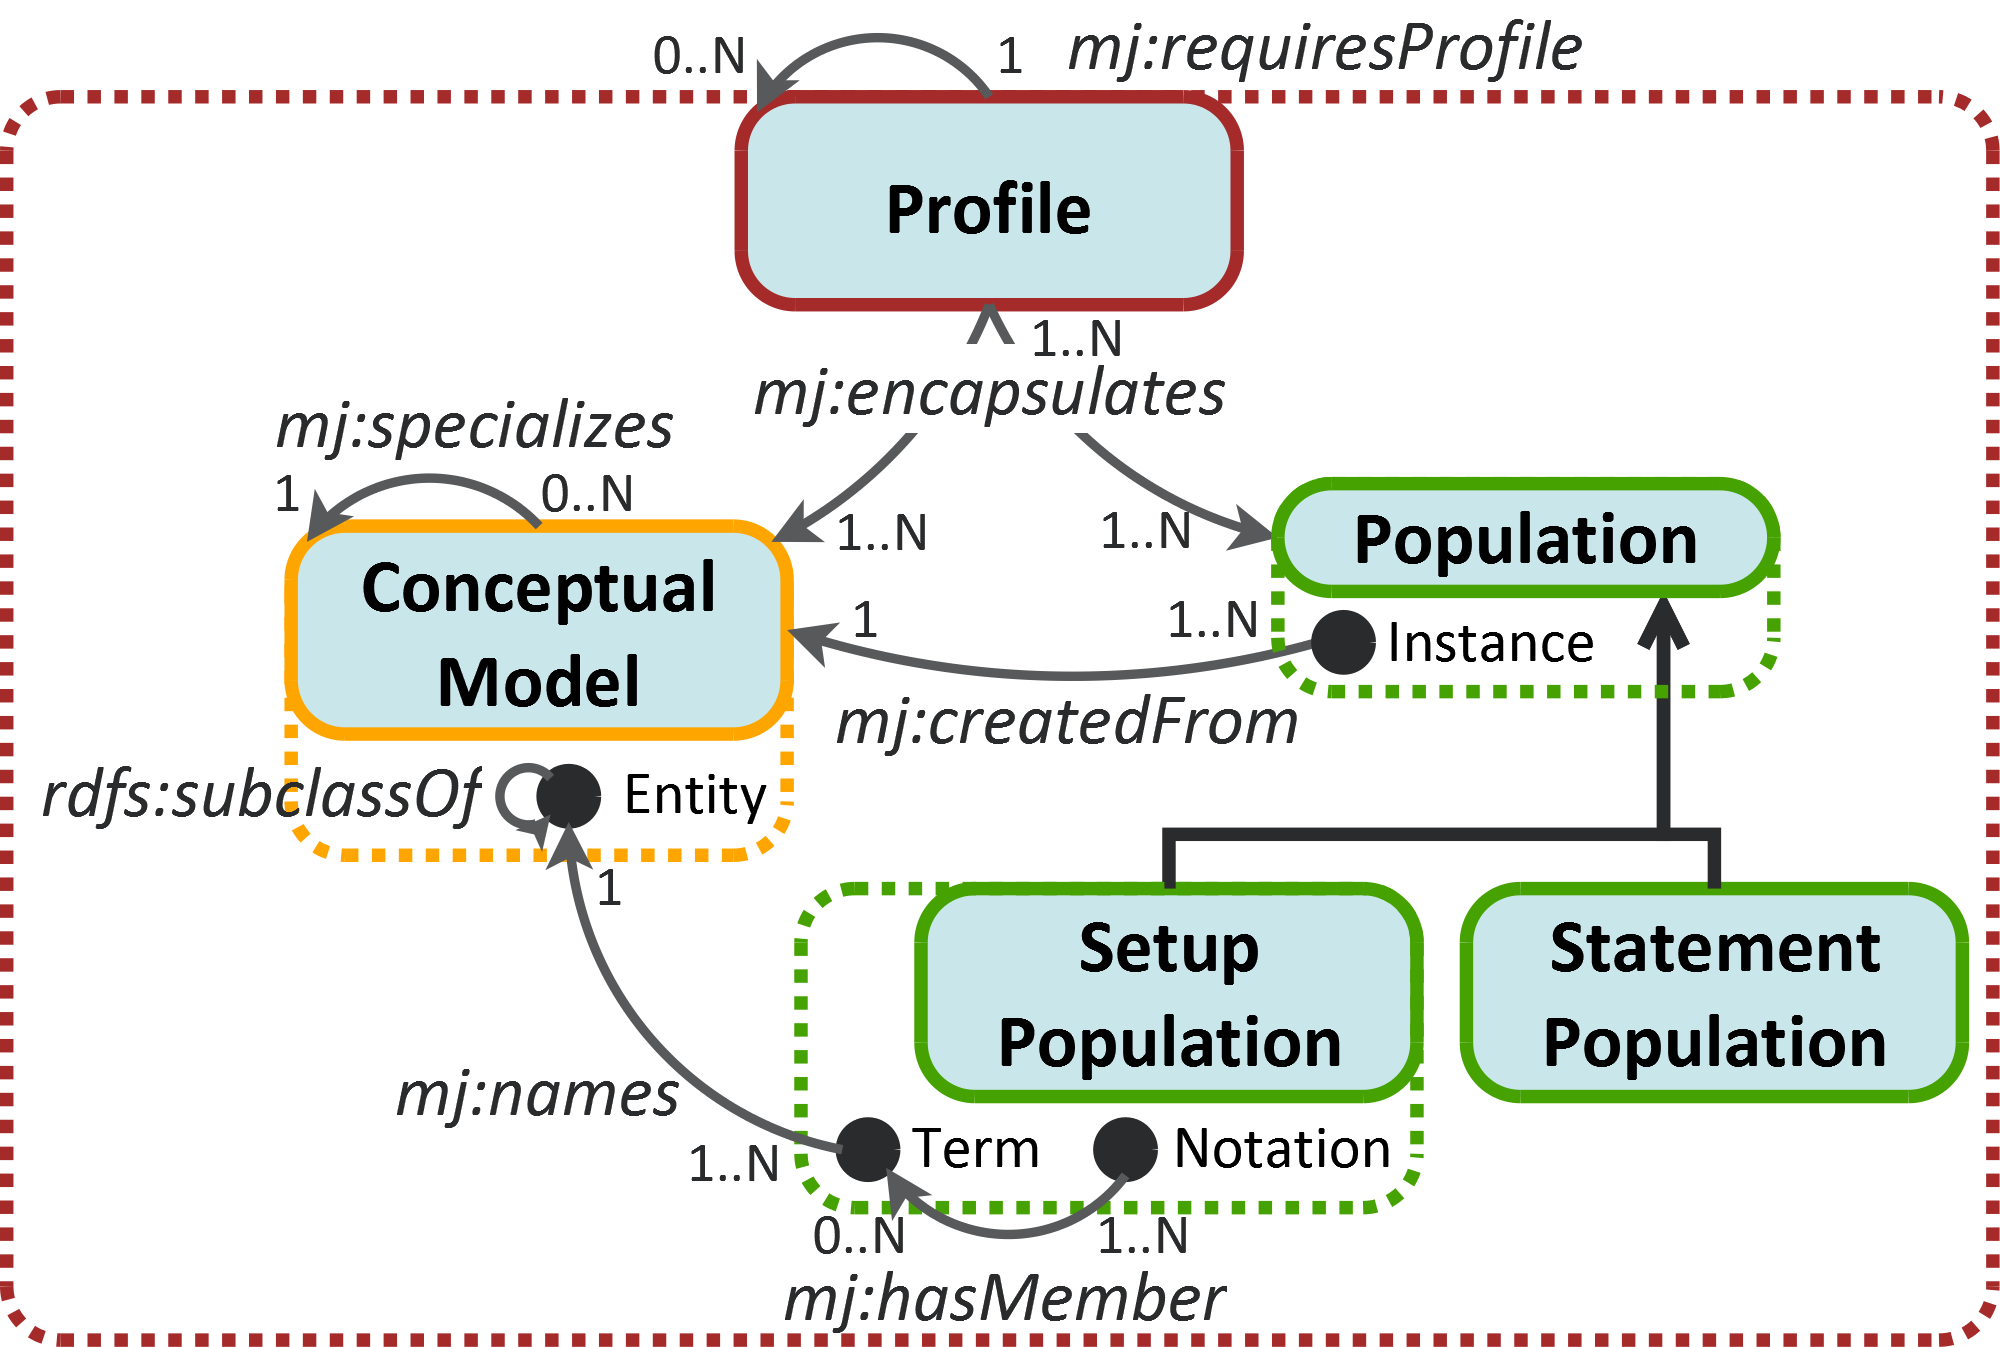
\includegraphics[width=0.7\textwidth]{./images/MOD-Profile-v3.png}
\caption{}
\label{img:conceptualisation}
\end{figure}


\subsubsection{Vue et contexte d'accès}\label{}

% \begin{cadrecol}{LightGoldenrodYellow}
% 	\con{} 
% \end{cadrecol}

\subsection{Le processus de production audiovisuelle}\label{}
\subsubsection{Projet, Produit, Contributeur}\label{}
\subsubsection{L'écriture audiovisuelle}\label{}


\subsection{Le document audiovisuel}\label{}
\subsubsection{Structure documentaire}\label{}
\subsubsection{Manifestations}




